\begin{enunciado}{15}
    The monotonically increasing hypothesis set is
    
    $$ \hipotset = \{ h~|~ x_1 \ge x_2 ~ \Rightarrow ~ h(x_1) \ge h(x_2) $$
    
    where $x_1 \ge x_2$ if and only if the inequality is satisfied for every component.
    
    \letra{a} Give an example of a monotonic classifier in two dimensions, clearly showing the $+1$ and $-1$ regions.

    	

    
    \letra{b} Compute $m_{\hipotset}(N)$ and hence the VC dimension. \textit{[Hint: Consider a set of $N$ points generated by first choosing one point, and then generating the next point by increasing the first component and decreasing the second component until $N$ points are obtained.]}

\end{enunciado}
    \letra{a} Resposta:
    
    Seja o seguinte classificador:

   $h(x_1, x_2)$ = 
    $
    \begin{cases}
	    +1 &\mbox{se } x_1 > \alpha \; \text{e} \; x_2 > \beta  \\ 
	    -1 &\mbox{caso contrário }
    \end{cases}
    $

    Essa classe de classificadores é monotonicamente crescente (Figura~\ref{fig:ex15a}).

    \begin{figure}[h]
	    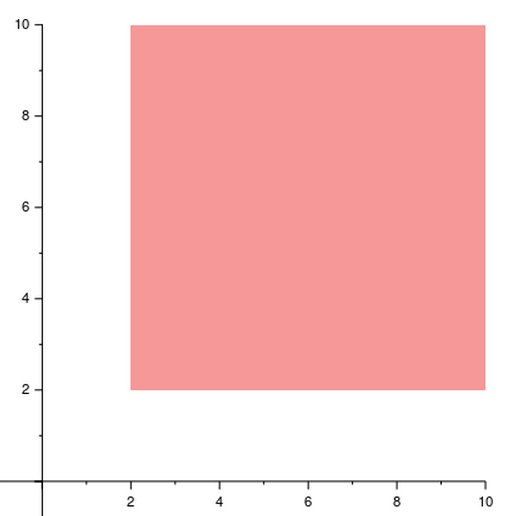
\includegraphics[width=0.3\textwidth]{ex15a}
	    \caption{Classificador monotonicamente crescente. A região colorida representa a classe +1.}
	    \label{fig:ex15a}
    \end{figure}
    
    \letra{b} Resposta:

    Construímos nosso conjunto de $N$ pontos do seguinte modo: dado um ponto $p_1$, o próximo ponto $p_2$ tem $x_1 > x_2$ e $y_1 < y_2$ (Figura~\ref{fig:ex15b}. Contamos o número máximo de dicotomias deste conjunto de pontos. Somamos o número de subconjuntos de tamanho 1, 2, \ldots, N. Dado nosso conjunto de pontos, nosso classificador não pode classificar o conjunto \{$p_1$ e $p_3$\} sem escolher $p_2$. Desse modo, deduzimos a função de crescimento, $m_{\mathcal{H}}(N) = \frac{N^2+N}{2}+1$. Logo, como $m_{\mathcal{H}}(2)=4$ e $m_{\mathcal{H}}(3)=7$, $\dvc=2$
    \begin{figure}[h]
	    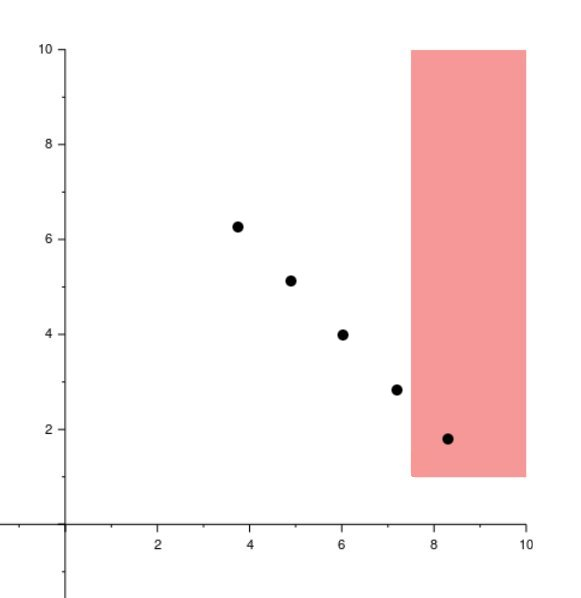
\includegraphics[width=0.3\textwidth]{ex15b}
	    \caption{Um exemplo de dicotomia}
	    \label{fig:ex15b}
    \end{figure}



